\chapter{A brief introduction to electric charges, currents, fields and potentials} 
\label{chap:Basics}
%%% fref fixed

Neural activity is generated by electric currents that go through neural membranes. In turn, these currents
evoke the extracellular electric potentials that are the main topic of this book. 

Before we talk more about the electric signaling in the brain, we will in this chapter give a general introduction to the physics of electricity. The aim of this rather incomplete introduction is to establish an elementary understanding of the main concepts that we will use in the remainder of this book. 

Most of the physics that we will go through is summarized in, and follows from, Maxwell's equations, and we might have kick-started this chapter by listing up those. However, since Maxwell's equations may appear a bit challenging for "the untrained eye", we will be taking a "softer" path, which we deem sufficient for establishing the main concepts that we will be working with. For good taste and later reference, we nevertheless go through Maxwell's equations in the final part of the chapter (Section \ref{sec:Basics:Maxwell}). Towards the end of the chapter we will also go through some of the most important assumptions that we use when applying the electromagnetic theory to predict electric potentials in complex medium like brain tissue.

Readers without prior schooling in physics will probably not be able to follow all parts of this introduction, but it will hopefully still give them a basic understanding of the concepts of \textit{electric charge}, \textit{electric currents}, \textit{electric fields}, and \textit{electric potentials}, and some insight into how they are related to one another. Readers that do have a physics background might see the first part of this introduction as a useful repetition, and may appreciate the later parts, which deal deals with less trivial issues regarding the use of electromagnetic theory in a complex medium such as brain tissue. 

\gen{Kanskje spesielt nevne noe om at folk med bakgrunn i fysikk ofte tenker paa hjernen som et dielektrikum (som ofte er tema i vanlige fysikkurs) og ikke som en conductor. En grunn til dette kan vaere at den matematiske formelen for potensialet rundt en stromkilde i en leder, er den samme som for potensialet rundt en ladning i et dielektrikum.}



\section{\blue{Electric charge}}
\label{sec:Basics:Charge} \index{Charge}
Let us begin with the fundamental quantity for electricity, the electric charge. Nature's fundamental charges are those carried by the protons and electrons that build up the atoms that build up the material world. The proton carries the charge $e$, while the electron carries the charge $-e$, where $e = 1.602\times10^{-19}$ coulomb (\si{\coulomb}) is called the \textit{unit charge} \index{Unit charge}. 
\gen{Endret Coulomb til coulomb, tror konvensjonen er  aa bruke stor forbokstav naar man skriver ut hele enheten. Eller?}

Since atoms contain an equal number of electrons and protons, most matter is electrically neutral. Some mediums are nevertheless conductive, which means that they contain so-called "free charge carriers" that may move through the medium. In an electric copper cable, such as that powering a lamp in a in a normal house, the free charge carriers are electrons that are not bound to specific locations (i.e., to specific copper atoms), but can move freely through the copper material. In an electrolyte solution, for example salt-water \gex{(saline?}), the free charge carriers are instead ions, i.e., atoms or molecules that have gained or donated one or several electrons, and therefore have become electrically charged. The saline solutions that fill the intracellular and extracellular space of the brain are such electrolytic solutions. Important charge carriers in the brain are sodium and potassium ions (Na$^+$ and K$^+$ with charge $1e$), chloride ions (Cl$^-$ with charge $-1e$), and calcium ions (Ca$^{2+}$ with charge $2e$).

At a fundamental, microscopic level, electricity is largely due to the interactions between individual charges. A pair of charges, $q_1$ and $q_2$, will act on each others with a force $F$ (with units newton (\si{\newton})) given by Coulomb's law:
\begin{equation}
F = \frac{q_1q_2}{4\pi \epsilon_0} \frac{1}{r^2}, 
\label{eq:Basics:CoulombF}
\end{equation}
where the constant $\epsilon_0$ is the permittivity of free space, and $r$ is the distance between the two charges. The direction of the force is along the line between the two charges, and the force is inversely proportional to the square of the distance between them. The force will be repelling if the charges have the same sign and attractive if they have the opposite sign.

We can express the direction of the force mathematically by use of a vector notation. Letting a boldface notation indicate that an entity is a vector, we denote the positions of the charges $q_1$ and $q_2$ by ${\bf r}_1$ and ${\bf r}_2$, respectively. The position vector ${\bf r}_1$ can be visualized as an arrow from some reference point $r=0$ \gen{Burde referansepunktet vaere beskrevet som en vektor ogsaa?} to the position of the charge $q_1$. Likewise, the vector ${\bf r}_1-{\bf r}_2$ can be visualized as an arrow from the position of $q_2$ to the position of $q_1$, defining both the distance and direction of the (imagined) line connecting them. In vector notation, the force between the charge pair can be written:
\begin{equation}
{\bf F} = \frac{q_1q_2}{4\pi \epsilon_0 |{\bf r}_1-{\bf r}_2|^2} \hat{{\bf r}}_{1,2}.
\label{eq:Basics:CoulombFvec}
\end{equation}
We have here introduced the \textit{unit vector}, defined as: 
\begin{equation}
\hat{{\bf r}}_{1,2} = \frac{{\bf r}_1 - {\bf r}_2}{|{\bf r}_1-{\bf r}_2|}, 
\label{eq:Basics:UnitVector}
\end{equation}
i.e., a vector ${\bf r}_1-{\bf r}_2$ divided by its own length $|{\bf r}_1-{\bf r}_2|$, so that its length is one (unity). We chose this notation because the unit vector then defines the direction of the force, but says nothing about its magnitude, while the fraction in front of the unit vector is a scalar (a number with no direction) that defines the magnitude of the force, but  says nothing about its direction. It is then easy to verify that the magnitude is the same as in \fref{eq:Basics:CoulombF}.

If there are several ($N$) point charges present, the contribution from each of them sum up linearly. If we have a charge $q_1$ in a position ${\bf r}_1$, the force acting on it by the $N-1$ other charges $q_2, q_3, q_4 ... q_{N}$ in positions ${\bf r}_2, {\bf r}_3, {\bf r}_4 ... {\bf r}_{N}$ will be:
\begin{equation}
{\bf F}({\bf r_1}) = \sum_{n=2}^{N} \frac{q_1 q_n}{4\pi \epsilon_0} \frac{\hat{{\bf r}}_{1,n}}{|{\bf r}_1-{\bf r}_n|^2}.
\label{eq:Basics:CoulombFN}
\end{equation}

If our system of study consisted of a small number $N$ of charges, we could use $N$ instances of \fref{eq:Basics:CoulombFN} to compute the force acting on all the $N$ individual charges. Together with Newton's law ${\bf F} = m {\bf a}$, which tells us how the charges will be accelerated in the force direction, \fref{eq:Basics:CoulombFN} would then allow us to compute the movements of all our charges over time. 

There is a fairly long way to go from \fref{eq:Basics:CoulombF} to the understanding of electric phenomena in a macroscopic system such as for example the brain. When describing a macroscopic system, we are usually not interested in the microscopic interactions between a small number of charges, but rather the joint interactions of a very, very large number of charges. It is then not feasible to keep track of the motion of each individual charge. At the larger scale, we therefore do not want to work with forces acting on individual particles, but rather with the concept of electric fields, which we will define below. It is still nice to have taken a look at \fref{eq:Basics:CoulombFN}, since it establishes the fundamental origin of electrical forces and fields. 
\gen{I tillegg kan det jo ogsaa vaere magnetiske krefter paa ladninger, kanskje bare nevne det for "completeness"?}


\section{\blue{Electric fields and potentials}}
\label{sec:Basics:Fields} \index{Electric field}

The electric field at a given location (with units volts per meter (\si{\volt\per\metre})) can be defined as the force that would act on a reference charge $q$ if it were present there, i.e., 
\begin{equation}
{\bf E}({\bf r}) = {\bf F}({\bf r})/q.
\label{eq:Basics:E}
\end{equation}
If we assume that this force is exclusively due to the Coulomb force, the electric field generated by $N$ charges can be obtained by inserting \fref{eq:Basics:CoulombFN} into \fref{eq:Basics:E}:
\begin{equation}
{\bf E}({\bf r}) = \sum_{n=1}^{N}  \frac{q_n}{4\pi \epsilon_0} \frac{\hat{{\bf r}}_{1,n}}{|{\bf r}-{\bf r}_n|^2}.
\label{eq:Basics:CoulombEN}
\end{equation}

Tightly related to the electric field ${\bf E}$ is the electric potential $\phi$ (with units volts (\si{\volt})), which is what we normally measure experimentally when we stick an electrode into the brain\index{Electric potential}. \gen{Senere har vi vel brukt andre symboler for potensial, i alle fall jeg}
While ${\bf E}$ is a fundamental physical entity, $\phi$ may be regarded as an auxiliary variable. It is a way to represent the electric field that often makes computations simpler and measurements easier. 

The electric field can be expressed as the spatial derivative, or gradient, of the potential:
\begin{equation}
{\bf E}(x,y,z) = - {\bf \nabla} \phi(x,y,z) = - \left(\frac{d\phi}{dx} {\bf e}_x  + \frac{d\phi}{dy} {\bf e}_y + \frac{d\phi}{dz} {\bf e}_z \right) \phi.
\label{eq:Basics:EV}
\end{equation}
The operator ${\bf \nabla}$ computes a property's spatial rate of change (also called the gradient) in the various spatial directions, and ${\bf e}_x$, ${\bf e}_y$ and  ${\bf e}_z$ are the unit vectors in the three spatial directions $x$, $y$ and $z$, respectively. 

For a spherical symmetric potential, 
\begin{equation}
{\bf \nabla} \phi(r) = \frac{d\phi(r)}{dr} {\bf \hat{r}}.
\label{eq:Basics:SphericalNablaPhi}
\end{equation}
Since the field contribution from each point charge is spherically symmetric around its position ($r_n$), the field in \fref{eq:Basics:CoulombEN} can thus be written as the gradient of the potential: 
\begin{equation}
{\phi}({\bf r}) = \sum_{n=1}^{N}  \frac{q_n}{4\pi \epsilon_0} \frac{\hat{{\bf r}}_{1,n}}{|{\bf r}-{\bf r_n}|}.
\label{eq:Basics:CoulombPhiN}
\end{equation}

Unlike ${\bf E}$, which is a vector-field \gen{bindestrek her? :-)}, $\phi$ is a scalar function \gen{scalar field?}, and as such, it tends to be easier to deal with. We note that \fref{eq:Basics:EV} rests on something called the \textit{quasi-static approximation} of Maxwell's equations, which we explain further in \fref{sec:Basics:Maxwell}. 


\subsection{\blue{Electric ground}}
\label{sec:Basics:Ground} 
To get an intuitive understanding of the relationship between ${\bf E}$ and $\phi$, it helps to consider an idealized one-dimensional scenario with a constant field in the $x$-direction. Then, \fref{eq:Basics:EV} simplifies to,
\begin{equation}
E = -\frac{d\phi(x)}{dx} = -\frac{\Delta \phi}{\Delta x} = -\frac{\phi(x_b)-\phi(x_a)}{x_b-x_a},
\label{eq:Basics:EV1D}
\end{equation}
where the first equality follows from the 1D-assumption, the second from the assumption that $E$ is constant, and the third is simply a definition of the second, where $x_b$ and $x_a$ may represent any two arbitrary points in space. For example, if $E = 1$ \si{\volt\per\metre}, and if the distance between our points $x_b-x_a$ is 1m, \fref{eq:Basics:EV1D} tells us that $\phi$ will be 1 \si{\volt} lower in $x_b$ compared to $x_a$ (\fref{fig:Basics:Ground}).

\begin{figure}[!ht]
\begin{center}
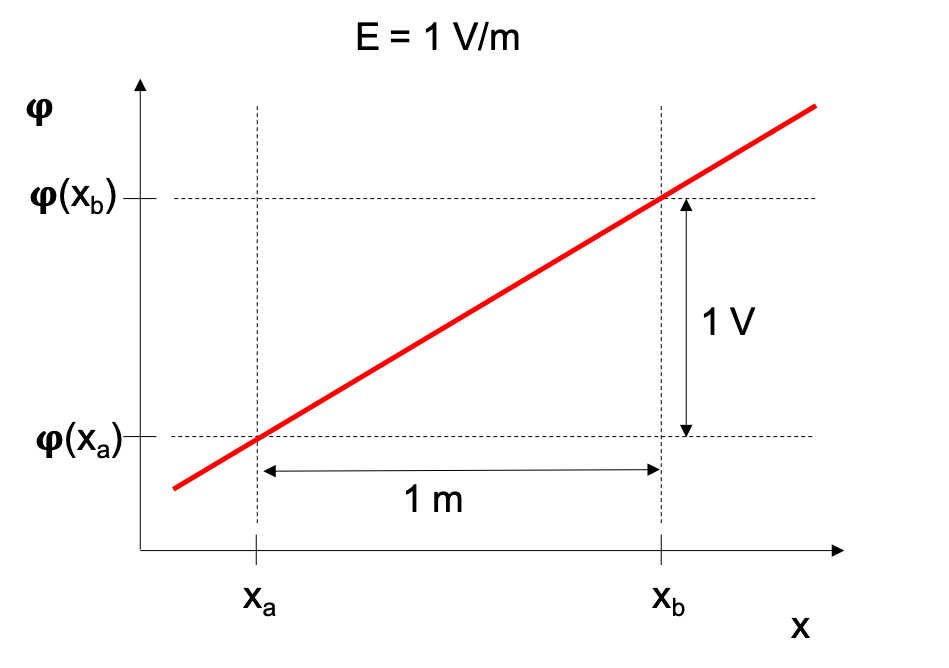
\includegraphics[width=0.8\textwidth]{Figures/Basics/Ground.png}
\end{center}
\caption{\textbf{Relationship between the electric field and electric potential.} With a constant electric field $E = 1\,\si{\volt\per\metre}$, the electric potential $\phi$ increases linearly with distance $x$. With two locations $x_a$ and $x_b$ 1 \si{\metre} apart, we know that $\phi(x_b) = \phi(x_a) + 1\,\si{\volt}$. We are free to define an arbitrary reference point (ground) for the $\phi$, and if we take $\phi(x_a) = 0$, it follows that $\phi(x) = (x-x_a)E$. In $x_b$, we then get $\phi(x_b)=(1\,\si{\metre})\times(1\, \si{\volt\per\metre}) =1\,\si{\volt}$. Equivalently, we might define $x_b$ as our reference point, which would mean that $\phi(x_b) = 0$ and $\phi(x_a) = -1\,\si{\volt}$. Regardless of where we place our reference point, the physics (i.e., the field, $E$) would be the same.
}
\label{fig:Basics:Ground}
\end{figure}

We may use the example in \fref{fig:Basics:Ground} to define the important concept of \textit{ground}\index{Ground}. The field ${\bf E}$ generally determines the potential only up to a constant. In the example, the field $E = 1$ V/m would be consistent with any pair of potentials $\phi_a$ and $\phi_b$ as long as $\phi_b - \phi_a =  1 \,\si{\volt}$. Since it is the field, and not the potential, that is the fundamental physical entity, we can therefore not speak of the potential in a certain point as an absolute entity, but only the potential \textit{difference} between two points. When we record potential in a given location, we must always record it relative to some an arbitrary reference point, which we call \textit{ground}, and where we define $\phi = 0$ (cf. example in \fref{fig:Basics:Ground}). 

When we record extracellular potentials, we can choose to place the reference electrode either outside or inside brain tissue \cite**{Sharott2015}, but we typically want to keep it at some distance from the recording electrode, so that reference electrode is not affected by the processes that we investigate with the recording electrode. \gen{Kanskje si enda klarere at man oensker at potensialet paa referanseelektroden skal vaere saa konstant som mulig under eksperimentet (eller blir dette sirkulaert?), husker at Anna plasserte referanseelektroden i nakken paa rottene hun gjorde maalinger fra. Kanskje vi kan hoere med eksperimentalistene paa CINPLA hva de gjoer?}

By definition, the electric potential is the energy needed to move a unit of electric charge $q$ from the reference point (ground) to a specific location in the electric field. The unit (V) of the electric potential is equivalent to energy per charge, or Joule per Coulomb (1 \si{\volt} = 1 \si{\joule\per\coulomb}). As such, the concept of an electric potential is closely related to the concept of a potential energy. The potential energy ($U_E$) of a charge $q$ in an electric field is:
\begin{equation}
U_E = q\phi.
\label{eq:Basics:UE}
\end{equation}


\subsection{\blue{Electroneutrality and Debye shielding}}
\label{sec:Basics:Debye} 
As the Coulomb force (\fref{eq:Basics:CoulombFN}) applies to a microscopic scale, so will the resulting electric field (\fref{eq:Basics:CoulombEN}) and potential (\fref{eq:Basics:CoulombPhiN}). The potential ${\phi}({\bf r})$ predicted from \fref{eq:Basics:CoulombPhiN} will therefore depend strongly on the distance to the nearest charge ($|{\bf r}-{\bf r_n}|$). Macroscopic media are normally densely packed with charges. For example, in the saline solution of the brain the average intra-charge distance is on the order of a nanometer, which means that the potential will vary strongly with a sub-nanometer resolution. A direct use of \fref{eq:Basics:CoulombPhiN} will therefore, again, force us to keep track of each individual charge, which would not be feasible in a macroscopic system.

Fortunately, we do not need to care too much about these microscopic field variations when we are trying to understand the brain.
\gen{Boer kanskje si noe om hvilke spoersmaal man da begrenser seg til? Er neglisjering av microscopic field variations det samme som aa anta
kontinuumapproksimasjon for elektrisk stroemmer? Og den kan generelt ikke brukes for detaljert modellering av stroem gjennom ionekanaler basert paa molekylaerdynamikk, slik jeg har forst{\aa}tt det.} A technical argument for why, is that the electrodes used to record brain signals have a tip diameter which is typically a micrometer or more. This is much larger than the average intra-charge distance in the saline solution of the brain. The electrodes therefore do not "sense" the microscopic fluctuations, but rather the average field taken over the electrode surface. 
\gen{"Surface" faar meg til kun aa tenke paa metallelektroder. Kanskje legge et ord eller to slik at liquid-elektroder ogsaa er dekket?} 
When we speak of an electric field or electric potential in the brain, we therefore always mean the field or potential on a so-called \textit{coarse-grained} scale, averaged over an electrode surface of at least 1 \si{\square\micro\metre}. A non-technical argument is that it is this coarse-grained signal, and not the microscopic reality that is bubbling underneath it, that is of importance if we want to understand the key brain processes. 

The Coulomb force (\fref{eq:Basics:CoulombF}) causes charges to attract charges of opposite valency and repel charges of the same valency. 
\gen{Omfatter ikke valency baade "sign" og antall elementaerladninger? Kanskje "sign" er bedre aa bruke her?} In a conductive medium, positive charges therefore tend to surround themselves with negative charges, and vice versa. Consequently, the numbers of positive and negative charges within a finite and not too small volume of space tend to be in close balance. On a coarse-grained scale, brain tissue will therefore to a good approximation be practically electroneutral \cite**{Nunez2006,Grodzinsky2011} \index{Electroneutrality}. If this was not the case, and a reference volume of tissue did contain a net charge density $\rho$, the very strong Coulomb-forces associated with it would cause $\rho$ to decay to zero at a rate proportional to the so-called \textit{charge-relaxation time}, which in brain tissue is on the order of a nanosecond (see \fref{sec:Basics:Quasimagnetostatic}).

The largest violation of electroneutrality occurs at neural membranes. \gen{Kanskje si eksplisitt at mens intracellular og ekstracellular "medium" kan sees paa som en "conductor", saa kan selve membranen sees paa som et isolerende dielektrikum (hvis en tenker paa vanlig elektrisk klassifisering av materialer)?}
Due to its capacitive properties (see \fref{sec:Basics:CapacitiveCurrent}), a patch of membrane can separate a charge $q$ on the interior side from a charge $-q$ on the exterior side. However, since the membrane is just some nanometers thick, also this charge separation occurs on a rather tiny spatial scale. On the coarse grained scale that we are interested in, we essentially consider entities averaged over volumes of tissue that are large enough to contain both intra- and extracellular components. Then electroneutrality will still be approximately preserved. 

The closely balanced negative and positive charges populating the tissue will tend to shield (cancel out) the electric fields from one another \gex{from the two types of charges?}, so that neither of them contribute to the field measured at some distance away from the charges. This phenomenon is known as Debye shielding \index{Debye shielding}. On a microscopic scale, we would expect a reference charge to evoke a potential given by the single charge version of \fref{eq:Basics:CoulombPhiN}, i.e., by:
\begin{equation}
\phi(r) = \frac{q}{4\pi \epsilon_0 r}.
\label{eq:Basics:Coulomb_phi1}
\end{equation}
However, according to \textit{Debye-H{\"u}ckel theory}, which we do not present in any detail here, the screening effects on a larger scale will cause the potential in an electrolyte to instead decay as:
\begin{equation}
\phi(r) = \frac{q}{4\pi \epsilon_0 \epsilon_r r} e^{-r/r_D}, 
\label{eq:Basics:DebyeScreening}
\end{equation}
where $r_D$ is called the \textit{Debye shielding distance} and $\epsilon_r$ is the \textit{relative permittivity} of the medium. 
\gen{Her kunne vi kanskje ogsaa oppgitt epsilon-r, som vel er 80 eller noe saant i vann?}
In the saline solution in the brain, $r_D$ is typically on the order of 8-9 \si{\angstrom} \cite**{Hille2001}, which implies that any given reference charge will give a negligible contribution to the potential at all macroscopic distances. 

The practical implication of electroneutrality and shielding effects is that, when we study extracellular potentials (or fields), we can neglect contributions from any particular distribution of charges, and instead compute extracellular potentials from the constraint that there should be no charge accumulation anywhere in the extracellular space. As we shall see, it will then be the current sources at neural membranes that give rise to an extracellular potential $\phi$. From here on, we shall thus not think of $\phi$ as something that we compute based on knowledge of the microscopic charge distribution (cf. \fref{eq:Basics:CoulombPhiN}), but rather as a higher level entity, exerting an average force on all charges in a certain direction. \gen{Si noe om at dette tilsvarer aa jobbe med ionekonsentrasjoner, istedenfor enkeltioner (hvis dette er riktig)?}


%%%%%%%%%%%%%%%%%%%%%%%%%%%%%%%%%%%%%%%%%%%%%%%%%
\section{\blue{Electric currents}}
\label{sec:Basics:Current} \index{Electric current}
As we have stated several times by now, we do not want to study a macroscopic system by keeping track of individual charges. We are instead interested in the electric currents, $I$ (units Ampere: \si{\ampere} = \si{\coulomb\per\second}), which represent the net movement of charge at a coarse-grained (space averaged) scale. There exist various kinds of electric currents, differing in terms of what drive them. Here, we will briefly introduce the three kinds that are most important for the topic of this book, the conductive current, the capacitive current and the diffusive current.

\subsection{\blue{Conductive currents}}
\label{sec:Basics:ConductiveCurrent} 
\index{Conductive current}
A conductive material  \index{Conductive medium} is one that charges can move through freely when they are exposed to an electric field. The conductive current is defined as the amount of charge that moves through some reference cross-section area per second. 

In electric circuits composed of wires and various circuit elements, currents are essentially one dimensional, running in the directions defined by the electric cables. The reference cross-section area is then typically taken to be that of "a whole cable", so that the current simply represents the total current through the cable. A simple example is shown in \fref{fig:Basics:Currents}A, where a current passes through a cable with a resistor. The current is then given by Ohm's law:
\begin{equation}
I = - \frac{\Delta \phi}{R}, 
\label{eq:Basics:Ohm_R}
\end{equation}
where $\Delta \phi = \phi_B-\phi_A$ is the voltage difference across the resistor, and $R$ (units Ohm (\si{\ohm})) its resistance. Here, the cable itself was assumed to have a zero resistance, so that the entire resistance in the system, and the entire voltage drop, was that over the resistor. To describe this system, we only needed to consider the potential at two locations, A and B, representing the two sides of the resistor. 

\begin{figure}[!ht]
\begin{center}
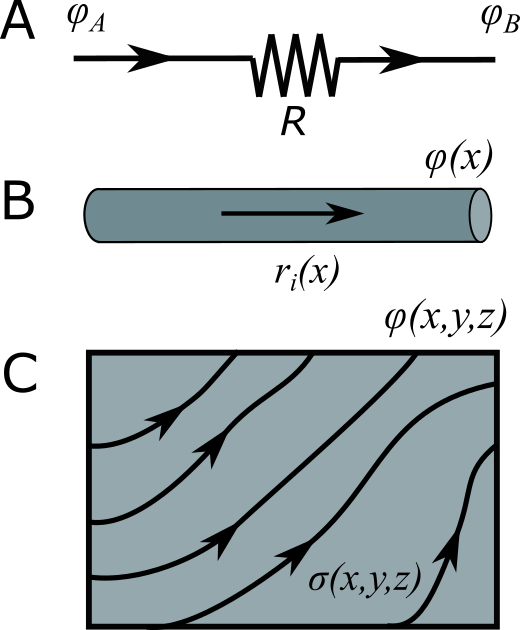
\includegraphics[width=0.6\textwidth]{Figures/Basics/Currents.png}
\end{center}
\caption{{\bf Ohms law for currents and current densities.} {\bf (A)} Current through cable with resistor with resistance $R$ (\si{\ohm}): $I = (\phi_B-\phi_A)/R$. {\bf (B)} Current in cable with specific axial resistance per unit length $r_a$ (\si{\ohm\per\metre}).  $I=- (1/r_a) d\phi/dx$. {\bf (C)} Current density (\si{\ampere\per\square\metre}) in a volume conductor with conductivity $\sigma$ (\si{\siemens\metre}): ${\bf i} = \sigma {\bf E} = - \sigma {\bf \nabla} \phi$.}
\label{fig:Basics:Currents}
\end{figure}

In reality, the resistance of the cable is not strictly zero, but for most standard electrical circuits it an excellent approximation. However, in some applications, for example for very long and thin cables, or for cables of less conducting materials, it may be necessary to treat cables as continuous resistors. If we define the specific axial resistance per unit length $r_{a}$ (units \si{\ohm\per\metre}, Ohm's law becomes: 
\begin{equation}
I = - \frac{1}{r_a}\frac{d\phi}{dx}, 
\label{eq:Basics:Ohm_r}
\end{equation}
where $r_a=r_a(x)$ may in principle vary along the cable (\fref{fig:Basics:Currents}B). With \fref{eq:Basics:Ohm_r}, the potential $\phi(x)$ will vary gradually along the cable. If $r_a$ is constant along the cable, and the cable has length $L$, it is related to the resistance of the total cable through $r_a=R/L$. Conductive currents running axially through neural dendrites and axons are typically modeled in this manner. 

The examples above were both one-dimensional in the sense that the current was restricted to run exclusively in the direction defined by the cable. In a three dimensional volume, such as for example brain tissue, currents may run in all spatial directions (\fref{fig:Basics:Currents}C). It is then convenient to describe them in terms of a current density, ${\bf i}$ (units \si{\ampere\per\square\metre}), a vector that defines the current per unit cross section area and its spatial direction. The current density can be defined in all points in 3D space, and is not dependent on any particular and predefined cross-section area. The conductive properties of a material can be specified either through its resistivity $r$ (units \si{\ohm\metre}), or its inverse, the conductivity $\sigma$ (units \si{\siemens\per\metre}), both being material properties. We shall here use the latter convention, and with that, Ohms law takes the form:
\begin{equation}
{\bf i} = - \sigma {\bf \nabla} \phi
\label{eq:Basics:Ohm_3D_phi}
\end{equation}

On a more general form, Ohms law states that:
\begin{equation}
{\bf i} = \sigma {\bf E}.
\label{eq:Basics:Ohm_general}
\end{equation}
In comparison, \fref{eq:Basics:Ohm_R}-\fref{eq:Basics:Ohm_3D_phi} hold only in the cases when the electric field ${\bf E}$ is conservative (cf. eq. \ref{eq:Basics:EV}), which we shall assume throughout this book. A discussion of this assumption is given in \fref{sec:VC:quasistatic}. We emphasize, however, that Ohms law applies specifically to \textit{conductive} currents, and that there exist other forms of electric currents not described by it.


\subsection{\blue{Capacitive currents}}
\label{sec:Basics:CapacitiveCurrent} 
\index{Capacitive current}
In the theory of electric circuits, a common circuit element is the capacitor. Capacitors are devices that can store electrical energy in terms of an electric field. The simplest form of a capacitor, a parallel plate capacitor, consists of two electrical metallic plates or surfaces separated by an insulating (dielectric) medium \index{Dielectric medium}.  By definition, a dielectric medium is one where charges are bound to stay in confined regions of space. An electric field only will slightly shift their average equilibrium positions, causing a polarization of the material. A parallel plate capacitor can separate a charge $q$ on one plate from a charge $-q$ on the other plate, to obtain a voltage difference:
\begin{equation}
\phi = \frac{q}{C}, 
\label{eq:Basics:Vcap}
\end{equation}
where $C$ (units Farad (\si{\farad} = \si{\coulomb\per\volt})) is the capacitance. 

To understand how a capacitor works, consider the illustration in \fref{fig:Basics:Capacitor}, where a conductive current $I^{in}$ enters the capacitor from the left, and a conductive current $I^{out}$ leaves to the right. Kirchhoff's current law states the current flowing into any node in a circuit must equal the current flowing out from that node, which means that we must define
a \textit{capacitive current} $I^{cap}$ over the capacitor, so that we get continuity: $I^{in} = I^{cap} = I^{out}$. 

\begin{figure}[!ht]
\begin{center}
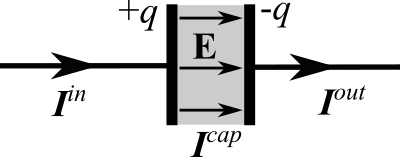
\includegraphics[width=0.6\textwidth]{Figures/Basics/Capacitor.png}
\end{center}
\caption{{\bf Capacitor}.  In the simplest form, a capacitor consists of two electrical metallic plates or surfaces separated by an insulating (dielectric) medium. Charges $q$ and $-q$ on the metal plate generate an electric field $E$ in the dielectric medium, or a potential difference, $\phi = Ed$ where $d$ is the distance between the metal plates. We skipped the vector notation on $E$ since the field direction is implicit.
}
\label{fig:Basics:Capacitor}
\end{figure}

Whereas the conductive currents $I^{in}$ and $I^{out}$ are mediated by charges moving freely through cables, no charges actually move across the capacitor itself. Instead, $I^{in}$ leads to an accumulation of charge $dq/dt$ on the left metal plate of the capacitor. This, in turn, evokes an electric field across its dielectric core, which drives positive charges away from the rightmost metal plate, charging it negatively $-dq/dt$. The temporal rate of change of the electric field across the dielectric medium can be described in terms of a capacitive current defined by:

\begin{equation}
I^\text{cap} = \frac{dq}{dt} = C\frac{d\phi}{dt}, 
\label{eq:Basics:Icap}
\end{equation}
Although $I^{cap}$ differs from conductive currents in the sense that it does not involve free transfer of charge through a medium, it has the same units (A). 

The capacitive current was introduced here because neural membranes have capacitive properties, which causes the neural membrane potential to change when currents pass through the membrane. It custom to express the capacitive membrane current in terms of a current density: 

\begin{equation}
i^\text{cap} = c_m\frac{d\phi_m}{dt}, 
\label{eq:Basics:Icap_mem}
\end{equation}
where $c_\text{m}$ (units \si{\farad\per\square\metre}) is the capacitance per unit membrane area. In this case, the current density is one-dimensional and in the direction normal to the membrane.


\subsection{\blue{Diffusive currents}}
\label{sec:Basics:DiffusiveCurrent} 
\index{Diffusion} \index{Diffusive current}
The charge carriers in the brain are ions floating around in the saline solutions that fill up the intra- and extracellular spaces. Ions in salt water will, like electrons in a metal conductor, be accelerated by the presence of an electric field, and will thus carry conductive currents. However, unlike electrons in the metal conductor, ions in water may also move due to diffusion. 

The electrodiffusive \index{Electrodiffusion} nature of ionic motion is described by the Nernst-Planck equation,
\begin{equation}
{\bf j_k} = - D_k {\bf \nabla} c_{k} - \frac{D_k z_k c_k}{\psi} {\bf \nabla} \phi,
\label{eq:Basics:JNP}
\end{equation}
which determines the flux density, ${\bf j_k}$ (units \si{\mole\per\square\metre\per\second}), of an ion species $k$. The first term on the right hand side of \fref{eq:Basics:JNP} is Fick's law for diffusion. It states that the diffusive flux of ion species $k$ is proportional to the diffusion constant ${D}_k$ (units \si{\square\metre\per\second}) times the concentration gradient ${\bf \nabla} c_{k}$. ${D}_k$ is generally a property of the medium that the ion diffuses through, and determines how "easy" it is for the ion $k$ to move through the medium. The second term on the right hand side of eq. \ref{eq:Basics:JNP} accounts for ionic drift due to the electric field. The factor $D_k/\psi$ is the electrical mobility of the ions, which is linearly related to their diffusion constant. This linear relationship is called the Einstein relation\index{Einstein relation}. It does not apply generally, but is valid for dilute solutions, such as the saline solutions in the brain \cite**{Grodzinsky2011}. The valency, $z_{k}$, is a unit-less number that denotes the number of unit charges associated with a single ion of species $k$. The factor $\psi=RT/F$ (units \si{\volt}) is defined by the gas constant ($R = 8.314 \, \si{\joule\per\mole\per\kelvin}$), Faraday's constant ($F = 96458.3\, \si{coulomb\per\mole}$), and the temperature ($T$ with units \si{\kelvin}). 

Faraday's constant is defined as the charge per mole ($1.602\times10^{-19}$) of unit charges. A flux density ${\bf j_k}$ can thus be converted to a current density by multiplying it with $Fz_k$. A salt water solution is composed of several ions, and to obtain the net electric current, we can sum over the contributions from all of them to obtain the total current density: 
\begin{equation}
{\bf i} = \sum_k z_k F {\bf j_k} = -\sum_k{F z_k {D_k}{\bf \nabla} c_{k}} - F\sum_{k} \frac{{D_k} z_{k}^2}{\psi}c_{k} {\bf \nabla}{\phi}.
\label{eq:Basics:iNP}
\end{equation}
The last term on the right hand side is the drift current density, 
\begin{equation}
{\bf i}^\text{drift} = - F\sum_{k} \frac{{D_k} z_{k}^2}{\psi}c_{k} {\bf \nabla}{\phi} = - \sigma {\bf \nabla}{\phi}.
\label{eq:Basics:idrift}
\end{equation}
As we indicated with the last equality, the drift current density is the same as the Ohmic current that we defined in eq. \ref{eq:Basics:Ohm_3D_phi}, which means that we can identify the conductivity $\sigma$ of a salt water solution as:
\begin{equation}
\sigma = \frac{F}{\psi}\sum_{k} {D}_k z_{k}^2 c_{k},
\label{eq:Basics:sigma_conc}
\end{equation}

The first term on the right hand side of \fref{eq:Basics:iNP} is the diffusive current density, 
\begin{equation}
{\bf i}^\text{diff}  = -\sum_k{F z_k {D_k}{\bf \nabla} c_{k}}.
\label{eq:Basics:idiff}
\end{equation}
Hence, in a conductive medium that contains concentration gradients, the total current is not purely Ohmic, but can contain an additional contribution from ionic diffusion. In many cases, the total current will be dominated by the drift component, and it is common to assume that the diffusive component is negligible. The diffusive current does, however, play an important role over neuronal membranes. 


\subsection{\blue{A note on Ohms law}}
\label{sec:Basics:Note} 
It is important to remember that Ohm's law (\fref{eq:Basics:Ohm_general}) represents the average movement of charge on a coarse-grained level, and does not apply on a microscopic scale. If we compare it with the microscopic fundament for this movement, it is easy to get confused, so let us dive into that confusion and try to clear it up. According to \fref{eq:Basics:E}, an electric field acts on a reference charge $q$ by a constant force, and should according to Newton's law (${\bf F} = m{\bf a}$) give it a constant acceleration in the field-direction. Conversely, \fref{eq:Basics:Ohm_general} states that ${\bf E}$ gives rise not to a constant acceleration of charges, but rather a constant current, i.e., a constant average \textit{velocity} of charges. 

The reason for the discrepancy between the microscopic (constant acceleration) and macroscopic (constant velocity) scales is that the constant acceleration (eq. \ref{eq:Basics:E}) at the microscopic level will go on for only a tiny time period (called the charge relaxation-time) \index{Charge-relaxation} before our protagonist charge $q$ will bump into some other particle and be scattered out in some random direction. After the scattering event, the acceleration will start "from scratch", and go on until the next collision takes place, and so forth. Whereas the scattering events will tend to make the motion of $q$ a random walk (which should give it a zero average velocity in any preferred direction), the small periods of acceleration between collisions will at average give $q$ a net drift velocity in the field direction. As the same will happen for all other charges present, there will be a net drift of charge in the field direction. The current density given by \fref{eq:Basics:Ohm_general} is therefore often referred to as the drift current density. Admittedly, the explanation that we proposed here was somewhat hand-waving, and the fact that we get the linear (constant velocity) relationship in \fref{eq:Basics:Ohm_general} is constitutive, meaning that it is observed experimentally rather than derived from first physical principles. It is found to be a good approximation for many mediums under many conditions, and it is an excellent approximation for brain tissue \cite**{Nunez2006,Pettersen2012}. 


\section{\blue{Extracellular potentials in the brain}}
\label{sec:Basics:ECSpot}
The main focus in this book is on modeling and interpreting extracellular potentials in the brain. Although these potentials fundamentally are due to the distribution of charges on a microscopic scale, the shielding effects that we discussed in  \fref{sec:Basics:Debye} allow us to predict the macroscopic (coarse-grained) extracellular potential from the constraint of that there should be no charge accumulation anywhere in the extracellular space, or equivalently, that there should be no net electric current entering or leaving any finite volume of tissue. We will start this endeavor by defining the types of currents that are relevant in different components of brain tissue. 

\subsection{\blue{Electric currents in the brain}}
\label{Basics:braincurrents}
Having introduced three different kinds of currents in \fref{sec:Basics:Current}, let us now summarize the role that they play within a brain-specific context. It is useful to make a distinction between currents existing in one of three different mediums, running through either: 
\begin{itemize}
\item The intracellular saline solution (cytosol)
\item The extracellular saline solution
\item The cellular (neuronal or glial) membrane
\end{itemize}

Among these three, the membrane currents are the odd ones out. A bit cartoonishly, we may think of the cellular membrane as an insulator (dielectric medium) with small holes. Due to its dielectric properties, it can store charges in so-called Debye-layers on its the in- and outside, in a way equivalent to how charges are stored on the metal plates in a parallel plate capacitor (cf. \fref{fig:Basics:Capacitor}). This charge-storage process can be described in terms of a capacitive current like that defined in by \fref{eq:Basics:Icap_mem}, which causes the membrane potential to vary with time. The holes represent various kinds of ion channels, which are conductive pores in the membrane that allow ions to pass through them. Ionic currents through the ion channels come in addition to the capacitive current. The capacitive and conductive membrane currents are both essentially one-dimensional and perpendicular to the membrane. They depend both voltage- and ion concentration differences between the inside and outside of the membrane, and are thus electrodiffusive in their nature, cf. \fref{eq:Basics:iNP}, but in one dimension, so that ${\bf \nabla} \rightarrow d/dz$. 

The intra- and extracellular currents are generally three-dimensional electrodiffusive volume currents (cf. \fref{eq:Basics:iNP}) through the conductive saline solutions that fill up the intra- and extracellular spaces. However, as concentration gradients within the intracellular and extracellular spaces typically are much smaller than those across membranes, it is common to neglect the diffusive component, and approximate that intra- and extracellular currents as being purely Ohmic (cf. \fref{eq:Basics:Ohm_3D_phi}). An illustration of the involved currents in a small piece of tissue is given in \fref{fig:Basics:Twostep}A. As indicated there, currents travel in loops, so that the intracellular and extracellular currents are coupled through the transmembrane currents at the boundary. Of course, there are infinitely many such loops in the system, and only a few were included in the illustration. 

For intracellular currents it is common to make the further simplification that they are well approximated as one-dimensional (cf. eq. \ref{eq:Basics:Ohm_r}). This is motivated by the morphological structure of neurons, which to a fair degree of accuracy can be represented as one-dimensional branching cables of varying diameter (\fref{fig:Basics:Twostep}B). 

\begin{figure}[!ht]
\begin{center}
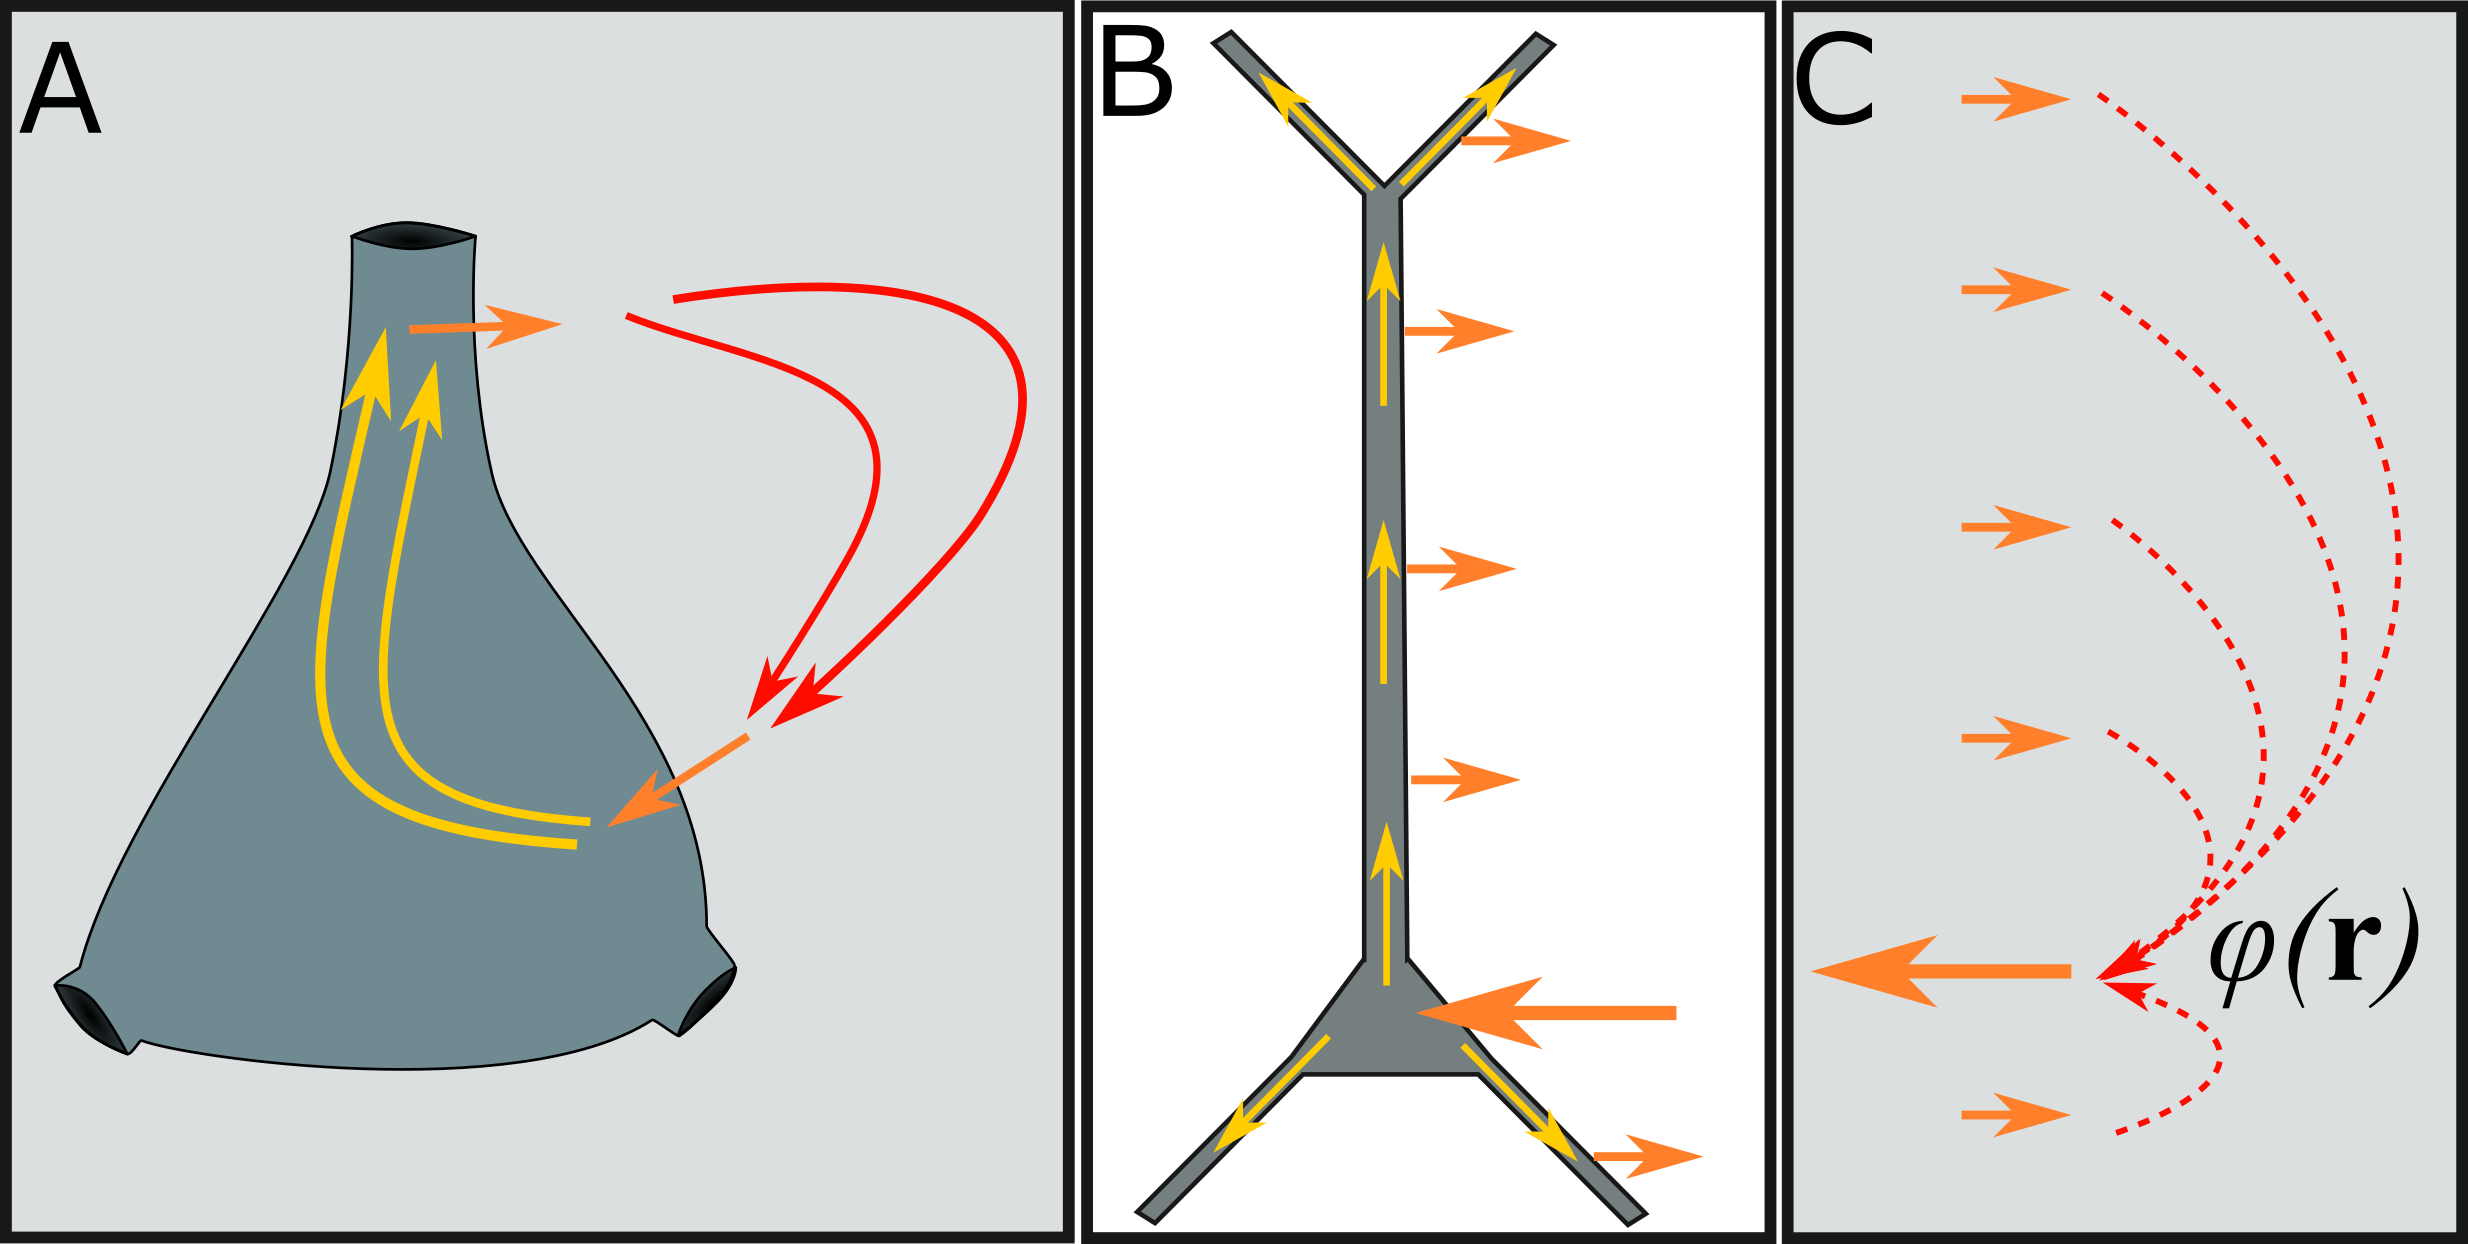
\includegraphics[width=1.0\textwidth]{Figures/Basics/Twostep.png}
\end{center}
\caption{{\bf Currents in brain tissue}. {\bf(A)} Illustration of currents involved in the brain, with intracellular volume currents (yellow), extracellular volume currents (red), and transmembrane currents (orange). Currents travel in closed loops. The entire space will be filled with currents, and only a paths was included in the illustration. {\bf(B)} A standard modeling strategy is to compute the intracellular and transmembrane currents on a framework independent of the extracellular dynamics. The neuron is approximated as a branching cable, and intracellular currents are one-dimensional along the cable, whereas transmembrane currents are perpendicular to the cable and distributed over the cable. {\bf(C)} The transmembrane currents computed in the framework {\bf(B)} can be used as output sources and sinks to the extracellular space, and can be used to compute the extracellular potential $\phi({\bf r})$. This will be the potential that is "needed" to complete all current loops. A few of which are illustrated with red, dashed arrows. 
}
\label{fig:Basics:Twostep}
\end{figure}


\subsection{\blue{Neurons as current sources}}
\label{sec:Basics:C} 
\index{Current source density}
It is custom to express current continuity in brain tissue in terms of a set of boundary conditions, where the boundaries are represented by the neuronal membranes. A common starting point for computing extracellular potential is the requirement that 
all currents entering or leaving through neuronal membranes must somehow be conserved and distributed in the extracellular space. This can be expressed mathematically through the continuity equation:
\begin{equation}
{\bf \nabla} \cdot {\bf i}_\text{t} = -C, 
\label{eq:Basics:continuity1}
\end{equation}
where the source term, $C$ (with units \si{\ampere\per\cubic\metre}), is called the current source density (CSD). The CSD represents the transmembrane output currents from neurons per tissue volume and includes both the capacitive and conductive membrane currents. We have let ${\bf i}_\text{t}$ denote the density of current running extracellularly through brain tissue. It does not include intracellular or transmembrane neural currents. 

In a volume of space where there is no neuronal membrane ($C = 0$), \fref{eq:Basics:continuity1} reduces to ${\bf \nabla} \cdot {\bf i}_\text{t} = 0$, which means that there will be no net tissue current entering or leaving such a volume. Importantly, this does not mean that the tissue current must be zero. Currents can still run \textit{through} the volume, as long as the amount of current entering it and leaving it are in balance. In a volume that \textit{does} receive a neuronal output, \fref{eq:Basics:continuity1} tells us that the current outputted from the neuron into that volume ($C$) must be carried away from that volume in terms of an extracellular tissue current. As we shall show in \Fref{chap:VC}, this conservation law shall be the fundament for modeling extracellular potentials surrounding active neurons.

For most parts of this book, we shall approximate brain tissue as a \textit{linear} Ohmic conductor, an approximation that we will discuss in further detail below. This means that the tissue current densities are given by \fref{eq:Basics:Ohm_3D_phi}. When this is inserted into \fref{eq:Basics:continuity1}, we obtain a relationship between the neuronal current sources and the extracellular potential: 
\begin{equation}
{\bf \nabla} \cdot \left(\sigma_\text{t} {\bf \nabla} {\phi} \right) = -C, 
\label{eq:Basics:continuity2}
\end{equation}
with $\sigma_\text{t}$ being the tissue conductivity. If $\sigma_\text{t}$ does not vary across space, this simplifies to the often used form:
\begin{equation}
\sigma_\text{t} \nabla^2{\phi} = -C.
\label{eq:Basics:continuity3}
\end{equation}


\subsection{\blue{Two-step approach for modeling extracellular potentials}}
\label{sec:Basics:twostep}
In order to compute extracellular potentials based on \fref{eq:Basics:continuity2}, we need to know the neuronal output $C$. Generally, the transmembrane currents in neurons depend on the membrane potential $\phi_\text{m}$, defined as the difference between the intracellular ($\phi_\text{i}$) and the extracellular ($\phi_\text{e}$) potentials immediately inside and outside the membrane. To compute intra- and extracellular potentials on a unified and spatially resolved framework is extremely computationally demanding, and unattainable for large systems. Standard modeling approaches are therefore based on the simplifying assumption that the neurodynamics is independent of whatever goes on in the extracellular space. One may then take a two-step approach to model the cellular and extracellular dynamics: 

\begin{itemize}
\item {\bf Step 1:} Compute the cellular dynamics (intracellular currents, membrane currents, and membrane potential) on a separate framework based on the assumption that this is independent on what goes on in the extracellular space (Fig. \ref{fig:Basics:Twostep}B). 

\item {\bf Step 2:} Use the transmembrane currents computed in Step 1 as "external" input $C$ to the extracellular space (Fig. \ref{fig:Basics:Twostep}C). Based on \fref{eq:Basics:continuity2}, with $C$ as obtained in Step 1, an analytical formula can be derived for how the set of transmembrane currents give rise to an extracellular potential $\phi({\bf r})$. 
\end{itemize}

Throughout this book, we shall use this two-step approach to compute extracellular potentials, but we will briefly introduce the theory behind alternative and more physically detailed frameworks. The standard framework for completing Step 1 is presented in \Fref{chap:Neuron}, and we will refer to it as the multicompartment (MC) framework, as it is based on multicompartment models of neurons. The standard framework for completing Step 2 is the volume conductor (VC) theory presented in  \Fref{chap:VC}. 


\section{\blue{Maxwell's equations}}
\label{sec:Basics:Maxwell} \index{Maxwell's equations}
Most of the physics that we have gone through so far follows from Maxwell's equations, so we will summarize this chapter by going briefly through these. We will also discuss some of the approximations of Maxwell's equations that we use when applying them to studies of brain tissue. 

Maxwell's equations come in two versions, referred to as the microscopic and macroscopic versions. The microscopic version is the most fundamental, but using it requires knowledge of the positions of all individual charges. Since that is unfeasible when any medium at a macroscopic level, we therefore only list up the macroscopic set of equations: 

\begin{eqnarray}
{\bf \nabla}\cdot {\bf D} & = & \rho. \label{eq:Basics:Max11} \\
{\bf \nabla} \cdot {\bf B} & = & 0.  \label{eq:Basics:Max22} \\
{\bf \nabla} \times {\bf E} & = & - \frac{\partial {\bf B}}{\partial t}.  \label{eq:Basics:Max33} \\
{\bf \nabla} \times {\bf H} & = & \bf{i^{free}} + \frac{\partial {\bf D}}{\partial t}.  \label{eq:Basics:Max44}.
\end{eqnarray}
Here $\rho$ and $\bf{i^\text{free}}$ are the free (unbound) charge and current densities, as the influence of bound charge and current is incorporated in the the auxillary displacement and magnetizing fields, ${\bf D}$ and ${\bf H}$. For linear mediums, ${\bf D}$ and ${\bf H}$ can be expressed in terms of the fundamental magnetic (${\bf B}$) and electric (${\bf E}$) fields through the constitutive relations ${\bf B} = \mu{\bf H}$ and ${\bf D} = \epsilon {\bf E}$, where $\mu$ (units henries per metre \si{\henry\per\metre}) is the magnetic permeability of the medium and $\epsilon$ (units \si{\farad\per\metre}) the electric permittivity of the medium. These linear approximations work well for brain tissue \cite**{Nunez2006}, and Maxwell's equations then take the form:

\begin{eqnarray}
{\bf \nabla}\cdot {\bf E} & = & \frac{\rho}{\epsilon}. \label{eq:Basics:Max1} \\
{\bf \nabla} \cdot {\bf B} & = & 0.  \label{eq:Basics:Max2} \\
{\bf \nabla} \times {\bf E} & = & - \frac{\partial {\bf B}}{\partial t}.  \label{eq:Basics:Max3} \\
{\bf \nabla} \times {\bf B} & = & \mu\bf{i}^\text{free} + \mu\epsilon\frac{\partial {\bf E}}{\partial t}.  \label{eq:Basics:Max4}
\end{eqnarray}

\Fref{eq:Basics:Max1} is Gauss's law (for electricity). The free charge density, $\rho$, can generally be non-zero, although we argued earlier that brain tissue for practical purposes can be assumed to be electroneutral at the coarse-grained scale. 

\Fref{eq:Basics:Max2} is Gauss's law for magnetism, and is the magnetic equivalent to eq. \ref{eq:Basics:Max1}. Whereas eq. \ref{eq:Basics:Max1} allows a spatial gradient of the electric field due to a local charge density $\rho$, eq. \ref{eq:Basics:Max1} disallows the corresponding gradient in the magnetic induction field. That is because magnetic monopoles do not exist. 

\Fref{eq:Basics:Max3} is the Maxwell-Faraday equation for electromagnetic induction. The cross product ${\bf \nabla} \times {\bf E}$ represents a certain kind of change in the electric field called the \textit{curl}. The equation tells us that such a change will be induced if there is a temporal variation in the magnetic field. 

\Fref{eq:Basics:Max4} is Ampere's circuital law, and is the magnetic equivalent to \fref{eq:Basics:Max3}. According to \fref{eq:Basics:Max4}, a magnetic field will be induced either by an electric current of free charges going through the medium (first term on the right), or by a temporal change in the displacement field (second term on the right). The last term is often called the displacement current. The Ohmic current that we introduced earlier (\fref{eq:Basics:Ohm_general}) is an example of a current of free charges, while the capacitive current that we introduced earlier (\fref{eq:Basics:Icap_mem}) is an example of a displacement current, where the capacitance can be expressed as a function of $\epsilon$. 

Together, Maxwell's equations give a unified theory for electricity and magnetism, and laid the theoretical fundament for understanding electromagnetic radiation such as light. We can "see the light" by looking at \fref{eq:Basics:Max3} and \fref{eq:Basics:Max4}. \Fref{eq:Basics:Max3} shows that a temporal change the magnetic field induces an electric field perpendicular to the change (perpendicular, because that is what the operation ${\bf \nabla} \times$ does), while \fref{eq:Basics:Max4} (last term) shows that a temporal change in the electric field induces magnetic field perpendicular to the change. Electromagnetic radiation is due to such an interplay where electric and magnetic fields act on each-others through a periodic series of inductions and cancellations that propagate as a wave through a medium. 

Another fundamental physical principle that follows from Maxwell´s equations is that of charge conservation. To see this, we may start with taking the gradient (${\bf \nabla} \cdot$) of both sides of eq. \ref{eq:Basics:Max4}. Since the gradient of a cross product is always zero, \fref{eq:Basics:Max4} then reduces to:
\begin{equation}
{\bf \nabla} \cdot \left( {\bf i}^\text{free} +  \epsilon \frac{\partial {\bf E}}{\partial t} \right) = 0.
\label{eq:Basics:Max4dot}
\end{equation}
This states that the sum of all currents (of free charges plus displacement) into any volume of space must be zero. To see the charge conservation explicitly, we can insert \fref{eq:Basics:Max1} for ${\bf E}$ to obtain:
\begin{equation}
- {\bf \nabla} \cdot {\bf i}\text^{free} =  \frac{\partial \rho}{\partial t},
\label{eq:Basics:currentconservation}
\end{equation}
Hence, if the left hand side in nonzero, there is a net influx of free charges into a volume, and if that is the case, there must be an accumulation of charge there, as described by the right hand side of the equation. This equation thus reveals that the displacement current can be expressed in terms of a local accumulation of free charge.


\section{\blue{Approximations used when studying brain dynamics}}
Throughout most of this book, we shall base our theory for computing extracellular potentials on \fref{eq:Basics:continuity2}, which rests on a series of approximations. Below, we go through the most important ones. 


\subsection{\blue{Quasi-electrostatic approximation of Maxwell's equations}}
\label{sec:Basics:Quasielectrostatic} \index{Quasi-electrostatic approximation}
As we have seen, electric fields can arise from both magnetic induction and from the presence of electric charges (cf. \fref{eq:Basics:Max1}). In the brain, this latter contribution is much larger than the contribution from magnetic field variations, and the electromagnetic radiation caused by the interplay between magnetic and electric fields does not play an important role for the workings of the brain. When studying brain processes, we therefore apply the so-called electro-quasi-static approximation of Maxwell's equations, which means that the temporal derivative of the magnetic field is set to zero.This means that eq. \ref{eq:Basics:Max3} simplifies to ${\bf \nabla} \times {\bf E} = 0$, which is a prerequisite for expressing ${\bf E}$ as a gradient of a potential (cf. \fref{eq:Basics:EV}). This assumption was also implicit when we expressed {\bf E} as a function of charges in \fref{eq:Basics:CoulombEN}.

\subsection{\blue{Quasi-magnetostatic approximation of Maxwell's equations}}
\label{sec:Basics:Quasimagnetostatic} \index{Quasi-magnetostatic approximation}
The right hand side of eq. \ref{eq:Basics:Max4} contains a total current,
\begin{equation}
{\bf i}^\text{tot} = {\bf i}^\text{free} + \epsilon\frac{\partial {\bf E}}{\partial t}, 
\label{eq:Basics:totcurrent}
\end{equation}
composed of a current of free charges (first term) plus a displacement current (last term). For an idealized conductor, the displacement current is zero, while for an idealized capacitor, the current of free charges is zero. 

Making the quasi-magnetostatic approximation means assuming that the displacement current, or equivalently, capacitive effects, are absent, so that \fref{eq:Basics:Max4} simplifies to ${\bf \nabla} \times {\bf B}  =  \mu{\bf i}^\text{free}$. This will be a good approximation provided that the magnitude ${\bf i}^\text{free}$ is much smaller than that of the displacement current. In the following, we will investigate the conditions for this to be a valid approximation. To simplify the analysis, we assume that the current of free charges is purely Ohmic, so that \fref{eq:Basics:totcurrent} becomes:
\begin{equation}
{\bf i}^\text{tot} = \sigma {\bf \nabla} \cdot {\bf E} + \epsilon\frac{\partial {\bf E}}{\partial t}, 
\label{eq:Basics:totcurrent2}
\end{equation}
Let us now consider an electric field that oscillates with some frequency $f$, 
\begin{equation}
{\bf E} = {\bf E}_{max} e^{j2\pi f \epsilon t}, 
\label{eq:Basics:Ecomponent}
\end{equation}
where $j$ here is the imaginary unit. If we insert this into \fref{eq:Basics:totcurrent2}, we get:
\begin{equation}
{\bf i}^\text{tot} = \sigma{\bf E} +  j 2 \pi f \epsilon {\bf E} = \left( \sigma + j 2 \pi f \epsilon \right){\bf E}
\label{eq:Basics:totcurrent3}
\end{equation}
From this it is clear that the capacitive contribution (last term) is negligible compared to the conductive contribution (first term) when the ratio
\begin{equation}
\frac{2 \pi f \epsilon}{\sigma} << 1. 
\label{eq:Basics:ratiocondition}
\end{equation}
Here, both $\sigma$ and $\epsilon$ can generally be functions of the frequency $f$. 

To gain some insight into the ratio $\epsilon/\sigma$, consider at the current conservation law (\fref{eq:Basics:currentconservation}), which when the current of free charges is purely Ohmic becomes:
\begin{equation}
\frac{\partial \rho}{\partial t} + \sigma {\bf \nabla} \cdot {\bf E} = 0
\label{eq:Basics:OhmicConcervation}
\end{equation}
If we insert \fref{eq:Basics:Max1} for ${\bf E}$, we may rewrite this as:
\begin{equation}
\frac{\partial \rho}{\partial t} + \frac{\sigma}{\epsilon} \rho = 0, 
\label{eq:Basics:OhmicConcervation2}
\end{equation}
which is a differential equation with the general solution
\begin{equation}
\rho({\bf r}, t) = \rho({\bf r}, 0)e^{-t/\tau}, 
\label{eq:Basics:relax}
\end{equation}
where we we have defined,
\begin{equation}
\tau = \frac{\epsilon}{\sigma}.
\label{eq:Basics:chargerelaxationtime}
\end{equation}
\Fref{eq:Basics:relax} shows that there is no steady-state free charge in the system considered. If any nonzero free charge occurs, for example due to sudden change in the electric field, it will decay towards zero with the time constant $\tau$, which is known as the charge-relaxation time \index{Charge relaxation}. If we insert for $\tau$, the criterion in \fref{eq:Basics:ratiocondition} simplifies to:
\begin{equation}
2 \pi f \tau << 1. 
\label{eq:Basics:ratiocondition2}
\end{equation}

Typical frequencies of interest for neural signals are on the order of 100 \si{\hertz}, which in an electromagnetic context can be considered a low frequency. Let us explore whether the criterion in \fref{eq:Basics:ratiocondition2} is met in three different mediums: 

\begin{itemize}
\item \textit{Extracellular saline solution:} The relative permittivity ($\epsilon_\text{r} = \epsilon/\epsilon_0$) of dilute salt water solutions, such as that filling up the extracellular space of the brain, is close to that of water, which at low frequencies is $\epsilon_\text{r} \sim 80$ \cite**{hasted1948}. The the extracellular solution has a conductivity $\sigma_\text{saline} \sim 2 \, \si{\siemens\per\metre}$ (see \fref{sec:Sigma}). This gives a value $\tau = \epsilon_r \epsilon_0/\sigma \sim 80\times 8.85\times10^{-12}/2 \simeq 0.35 \, \si{\nano\second}$. A charge relaxation time in the order of 1 \si{\nano\second} has also estimated in other works \cite**{Grodzinsky2011,Gratiy2017}), and implies that the displacement current will mainly be important under conditions when the electrical field varies with frequencies in the gigahertz range. The relevant fields with physiological origin vary with frequencies that are orders of magnitude lower than this ($f \sim 100 \, \si{\hertz} $), which implies that capacitive effects can safely be neglected. With $\tau = 0.35 \, \si{\nano\second}$ and $f = 100 \, \si{\hertz}$, $2 \pi f \tau =  2.2 \times 10^{-7}$, and the criterion in \fref{eq:Basics:ratiocondition2} is clearly met.

\item \textit{Neural membrane:} Neural membranes typically have a time constant $\tau \sim 1 \, \si{\milli\second}$ associated with their capacitive charging. This is much lower than the corresponding charge relaxation time of the extracellular saline solution. With $\tau = 1 \, \si{\milli\second}$ and $f = 100 \, \si{\hertz}$, $2 \pi f \tau =  0.63$, and the criterion in \fref{eq:Basics:ratiocondition2} is not met. Hence, capacitive current is an important contributor to the total membrane current.

We note that both the conductivity and capacitance of the membrane can be expressed in terms of the permittivity through the relations $\epsilon = c_m \Delta r$ and $\sigma = \epsilon / \tau$. Neural membranes typically have a specific membrane capacitance of $c_m \sim 10^{-2} \, \si{\farad\per\square\metre}$, a thickness $\Delta r \sim 10^{-8}\, \si{\metre}$, and a time constant $\tau \sim 10^{-3} \, \si{\second}$ \cite**{Nunez2006}. This amounts to a permittivity of $\epsilon \sim 10^{-10} \,\si{\farad\per\metre}$, and conductivity of $\sigma \sim 10^{-7} \, \si{\siemens\per\metre}$, although the latter can vary quite much depending on which ion channels that are present and activated. Both are lower than for the tissue medium, but the conductivity more so, resulting in a $\tau$ that is much bigger for the membrane than for the extracellular solution. 

\item \textit{Neural tissue:} As a third medium, we consider the neural tissue as a whole. Data from \citeasnoun**{gabriel1996compilation} suggests that grey matter has a relative permittivity $\epsilon_r \sim 10^6$ and conductivity $\sigma \sim 0.1 \, \si{\siemens\per\metre}$ at $f = 100 \, \si{\hertz}$. This gives a relaxation time constant $\tau = \epsilon_r \epsilon_0/\sigma \sim 10^6\times 8.85\times10^{-12}/0.1 \simeq 0.1 \, \si{\milli\second}$. With this value, we get $2 \pi f \tau =  0.06$. This is much larger than for the extracellular saline solution, and reflects the fact that currents passing through tissue will not solely be in contact with the saline solution, but may also interact with neural membranes. Nevertheless, the relative contribution of the capacitive current is fairly low also in tissue, meaning that Ohmic currents will dominate. We note that there is quite some variation in experimental estimates of  $\epsilon_r$ and $\sigma$ for the tissue medium, but they are normally of the same order of magnitude as the values used in the calculation above.
\end{itemize}

In conclusion, the quasi-magnetostatic approximation seems justified for currents through tissue and in the extracellular saline solution, but not for transmembrane currents.


\subsection{\blue{Extracellular currents are exclusively due to electric drift}}
\label{sec:Basics:onlyohmic}
When analyzing extracellular currents in the brain, it is common to assume that they are purely due to electric drift, as we do when using the volume conductor (VC) theory that we present in \Fref{chap:VC}. In principle, a current could have additional contributions from ionic diffusion, advection currents, displacement currents, and electromagnetic induction, so that the total current density would be:
\begin{equation}
{\bf i} = {\bf i}^{ohm} + {\bf i}^{diff} + {\bf i}^{adv} + {\bf i}^{dis} + {\bf i}^{ind}, 
\label{VC:eq:generalcurrent}
\end{equation}

As the displacement current is proportional to $\partial {\bf E}/\partial t$, and the inductive currents is proportional to $\partial {\bf B}/\partial t$, it follows from the quasi-magnetoostatic and quasi-electroostatic approximations, respectively, that they are zero. 

An advective current \index{Advective current}, 
\begin{equation}
{\bf i}^{adv} = F \rho {\bf u}, 
\label{VC:eq:iadv}
\end{equation}
arises in a bulk solution if the solution has a charge density $\rho$ that it drags along with it due to a bulk flow with velocity ${\bf u}$. As we argued in \fref{sec:Basics:Debye}, the extracellular medium is practically electroneutral ($\rho \simeq 0$), and the advective current therefore becomes negligible. A more thorough argument for this was given in \citeasnoun**{Gratiy2017}. 

The diffusive current \index{Diffusive current},
\begin{equation}
{\bf i}^{diff} = -F \sum_k z_k D_k {\bf \nabla} c_k,
\label{VC:eq:idif}
\end{equation}
arises when ions (with valence $z_k$ and diffusion constants $D_k$) diffuse along concentration gradients (${\bf \nabla} c_k$), and carry with them a net charge. It has been suggested that diffusive currents can have a notable impact on $\phi$ in physiological conditions with large concentration gradients \cite**{Halnes2016}, especially if ion concentration gradients vary quite rapidly with time \cite**{Gratiy2017}. Diffusive effects on $\phi$ may therefore be particularly relevant under pathological conditions such as epilepsy, stroke and spreading depression, which are associated with dramatic shifts in local extracellular concentrations (see e.g.,  \cite**{Somjen2001,Frohlich2008,Wei2014,Ayata2015}). 

To account for diffusive effects, one needs to compute not only the electrical potential, but also the ion concentration dynamics of all involved ions at all points in space. This can not be done using VC theory in the standard form presented in \Fref{chap:VC}, but can be done using Finite Element Methods (see e.g., \cite**{Solbra2018}). We go through the theory for modeling electrodiffusive systems in \fref{sec:Eldiff}.

Under normal conditions, drift currents are likely to have a much bigger impact on the time course of $\phi$ than diffusive currents. Standard VC theory, which neglects diffusive effects, will likely make quite good predictions of $\phi$ under most experimental conditions \cite**{Halnes2016,Gratiy2017}. 


\subsection{\blue{Linear extracellular medium} }
\label{sec:Basics:LinEx}
\index{Extracellular medium! Linear}
In practice, most medias can have capacitive, magnetic and conductive properties, and can be linear or nonlinear in all these three senses. Starting out with Maxwell's equations on the form given by \fref{eq:Basics:Max1}-\fref{eq:Basics:Max1}, we assumed linearity in the capacitive and magnetic sense, through the constitutive relations ${\bf B} = \mu{\bf H}$ and ${\bf D} = \epsilon {\bf E}$. 

Linearity in the conductive sense implies that the current density is linearly related to the electric field through Ohm's law:
\begin{equation}
{\bf i} = \sigma {\bf E}.
\label{eq:Basics:bertil}
\end{equation}

Ohm's law is quite general, and $\sigma$ can here in principle be anisotropic (i.e., a tensor, accounting for different conductivities in different directions) and inhomogeneous (position dependent). Furthermore, Ohms law does not exclude capacitive effects, because, for a medium that is linear in both the conductive and capacitive sense, capacitive effects can be incorporated into  \fref{eq:Basics:bertil} through defining a complex conductivity \cite**{Nunez2006}:
\begin{equation}
\sigma_c = \sigma(f)\left(1+j\frac{2\pi f \epsilon(f)}{\sigma(f)}  \right), 
\label{eq:Basics:complexsigma}
\end{equation}
where $j$ is the imaginary unit and $f$ the oscillation frequency of the electric field (or a component of it). Both the real and imaginary parts of $\sigma_c$ can be frequency dependent, and the two terms correspond to the conductive and capacitive properties of the medium, respectively. 

The current density in \fref{eq:Basics:complexsigma} comprises both the electric drift current and the displacement current. In this book, we will not use \fref{eq:Basics:complexsigma}, but keep the two current types separate, as we did in \fref{sec:Basics:onlyohmic}). Furthermore, for extracellular tissue currents we have argued that the capacitive effects are negligible, so that they are determined by \fref{eq:Basics:bertil} with a real $\sigma$. As we also make the quasi-electrostatic approximation of Maxwell's equations (\fref{sec:Basics:Quasielectrostatic}), ${\bf E}$ can be written as the gradient of an electric potential, so that the extracellular drift current density is given \fref{eq:Basics:Ohm_3D_phi}, and so that we can take \fref{eq:Basics:continuity2} as our starting point when deriving the VC theory in \Fref{chap:VC}.

We note that \fref{eq:Basics:bertil} is generally only valid in the frequency domain, while in the time domain, ${\bf i}$ must be given as a temporal convolution of $\sigma$ and ${\bf E}$ \cite**{Bedard2009}. However, if $\sigma$ is frequency independent (this assumption is discussed further in \fref{sec:Sigma}), \fref{eq:Basics:bertil} will also be valid in the time domain.


\subsection{\blue{Neurons as current sources} }
As we will use \fref{eq:Basics:continuity1}:
\begin{equation}
{\bf \nabla} \cdot {\bf i_t} = -C.
\label{eq:Basics:Greta}
\end{equation}
as our fundamental equation for modeling extracellular potentials, it worth making the effort of showing how it relates to general current conservation. To do this, we state the current conservation equation (\fref{eq:Basics:Max4dot}) on the form:
\begin{equation}
{\bf \nabla} \cdot \left( {\bf i}^{free} +  \epsilon \frac{\partial {\bf E}}{\partial t} \right) = {\bf \nabla} \cdot {\bf i}^{tot}  = 0, 
\label{eq:Basics:Melpomene}
\end{equation}
where we defined everything inside the parenthesis (free plus capacitive current) as the total current to keep notation short. 

The simplest way from eq. \ref{eq:Basics:Melpomene} to eq. \label{eq:Basics:Greta} may be to express the total current as being composed of a part ${\bf i}^{tot}_p$, which covers all intracellular and membrane currents, and a part ${\bf i}^{tot}_t$, which covers the currents that run extracellularly through tissue. Eq. \ref{eq:Basics:Melpomene} can then be written
\begin{equation}
{\bf \nabla} {\bf i}^{tot}_t = - {\bf \nabla} \cdot {\bf i}^{tot}_p.
\label{eq:Basics:Melpomene2}
\end{equation}

Cellular and extracellular currents do not exist at the same points in space, and on a microscopic scale,  only one of them will be nonzero at a given position. Hence, eq. \ref{eq:Basics:Melpomene2} only makes sense on a coarse-grained scale, where ${\bf i}^{tot}_p$ and ${\bf i}^{tot}_t$ represent the currents averaged over a finite piece of tissue, large enough to contain both types. On such a coarse-grained scale, the right hand side of eq. \label{eq:Basics:Melpomene2} can be expressed as a current source density ${\bf \nabla} \cdot {\bf i}^{tot}_p = C$, i.e., the cellular current output per unit volume of tissue, which brings us back to eq. \ref{eq:Basics:Greta}. This was shown by \citeasnoun**{Gratiy2017}, who performed a a spatial averaging over all the intracellular and membrane currents (i.e., over ${\bf i}^{tot}_p$ ) within a finite piece of tissue. The derivation (not shown here), reveals that eq. \ref{eq:Basics:Greta} only has a meaningful interpretation when considering tissue in a coarse grained scale.

